\documentclass[twocolumn,prb,showpacs,superscriptaddress]{revtex4}
\usepackage{graphicx}
\usepackage{amsmath}    % need for subequations

%
% warning: if you redefine \r you will have troubles with the angstrom,
% which is internally defined as \r{A}
%

\def\w{\omega}
\def\wp{\omega^\prime}
\def\wc{{\omega_{\rm C}}}
\def\>{\rangle}
\def\<{\langle}
\def\H{\hat{H}}
\def\P{\hat{P}_{\rm occ}}
\def\E{\varepsilon}
\def\vp{{v^\prime}}
\def\q{{\bf q}}
\def\s{\sigma}
\def\k{{\bf k}}
\def\qp{{\bf q^\prime}}
\def\G{{\bf G}}
\def\Gp{{\bf G^\prime}}
\def\rt{\tilde{r}}
\def\pt{\tilde{p}}
\def\r{{\bf r}}
\def\rp{{\bf r^\prime}}
\def\rpp{{\bf r^{\prime\prime}}}
\def\rppp{{\bf r^{\prime\prime\prime}}}
\def\mo{$\overline{1}$}
\def\mt{$\overline{2}$}

% -------
\usepackage{soul}
\usepackage{color}
\definecolor{yellow}{rgb}{1,1,0}
\definecolor{lightblue}{rgb}{0.6,0.6,0.9}
\sethlcolor{yellow}
% -------

\begin{document}

\title{GW method using density-functional perturbation theory}

\author{Feliciano Giustino}
\email{feliciano.giustino@materials.ox.ac.uk}
\affiliation{Department of Materials, University of Oxford, Parks Road, Oxford OX1 3PH, United Kingdom}
\affiliation{Department of Physics, University of California at Berkeley, 
Berkeley, California 94720, USA,
and Materials Sciences Division, Lawrence Berkeley National Laboratory, 
Berkeley, California 94720, USA}
\author{Marvin L. Cohen}
\author{Steven G. Louie}
\affiliation{Department of Physics, University of California at Berkeley, 
Berkeley, California 94720, USA,
and Materials Sciences Division, Lawrence Berkeley National Laboratory, 
Berkeley, California 94720, USA}
\date{\today}

\begin{abstract}
We propose a new approach to quasiparticle GW calculations which 
is based on density-functional perturbation theory and
does not require the calculation of unoccupied electronic states. The screened Coulomb interaction
is evaluated by solving self-consistent linear-response Sternheimer equations,
and the noninteracting Green's function is evaluated by solving inhomogeneous 
linear systems. The frequency-dependence of the screened Coulomb interaction 
is explicitely taken into account by performing calculations along the imaginary
frequency axis and then using Pad\'e approximants for the analytical continuation
to real frequencies. As a proof of concept we implemented the proposed method 
within the empirical pseudopotential formalism and we studied silicon as a test case. 
\end{abstract}

\pacs{71.15.-m, % Methods of electronic structure calculations
      71.15.Qe} % Excited states: methodology

\maketitle

\section{Introduction}

During the past two and a half decades the $GW$ method\cite{hedin1,hl86}
for the study of electron quasiparticle excitations
accomulated a number of successes and witnessed a significant growth of interest
within the computational electronic structure community.
The $GW$ method is currently being used for predicting electron quasiparticle
excitation spectra as well as optical spectra in a variety of materials
ranging from bulk solids to nanostructures and organic systems. The
$GW$ method is also of widespread use as a starting point for Bethe-Salpeter calculations
of two-particle neutral excitations.\cite{onida,rolfing,reining-review}
Current implementations find many diverse applications,
including among others the simulation of the optical response of nanostructures,\cite{catalin} quantum transport in nanoscale
junctions,\cite{rubio} pump-probe spectroscopy,\cite{catalin-lw} angle-resolved photoemission
spectroscopy,\cite{cheolhwan} and strongly-correlated systems.\cite{bruneval-oxide}

Current trends in the development of improved computational approaches for
quasiparticle excitations based on the $GW$ method include the refinement
of the initial guess for the non-interacting Green's function and for the
polarization operator,\cite{rinke,schilfegarde}
the inclusion of approximate vertex corrections or higher-order self-energy
diagrams\cite{york} and the description of the frequency-dependent
dielectric response beyond the original plasmon-pole approximation.\cite{spacetime,blochl}
Detailed reviews of past and current developments in $GW$ techniques can be
found in Refs.\ \onlinecite{hl,gunnarsson,reining-review,rinke}.

The majority of current implementations obtain the screened Coulomb interaction
$W$ and the non-interacting Green's function $G$ by using a perturbative
expansion over the Kohn-Sham wavefunctions (cf. Sec.\ \ref{sec.coulomb}). This expansion
requires the calculation of both occupied and unoccupied electronic states,
as well as their associated optical matrix elements.\cite{hl86} A common bottleneck 
of this approach is that the convergence of the results with the number $N_{\rm c}$ 
of unoccupied states is rather slow.\cite{sohrab} This is especially true for
the absolute values of the quasiparticle excitation energies.\cite{bruneval-gonze}
%
Several avenues have been explored so far in order to circumvent such bottleneck 
and to perform $GW$ calculations by employing occupied electronic states only,\cite{reining-sternheimer,umari1,umari2,gygi}
or only a limited number of unoccupied states.\cite{bruneval-gonze}


The main aim of the present work is to demonstrate the feasibility of $GW$ calculations
entirely based on density functional perturbation theory (DFPT).\cite{baroni.rmp}
In practice we adopt the principles of DFPT in order to (i) determine 
the {\it frequency-dependent screened Coulomb interaction} directly
by solving self-consistent linear response Sternheimer equations,
and (ii) to determine the non-interacting Green's function by solving
inhomogeneous linear systems. The main advantage of the proposed method 
is that it does not make use of unoccupied electronic states.
Additionally we investigate the possibility of fast evaluations of 
the frequency dependence of the screened Coulomb interaction
based on {\it multishift} linear-system solvers.\cite{frommer}
%
As a proof of concept we have implemented the method within
a planewaves empirical pseudopotential approach,\cite{cohen_berg} 
and tested it for the case of silicon.

The uses of the Sternheimer equation for calculating the polarizability
in the random-phase approximation (RPA) or the inverse dielectric matrix 
have already been discussed in Refs.\ \onlinecite{fleszar-resta,kunc-tosatti} 
within the context of supercell calculations. After the introduction 
of DFPT in the context of lattice-dynamical calculations,\cite{giannozzi} 
the authors of Ref.\ \onlinecite{reining-sternheimer} proposed the
use of the non self-consistent Sternheimer method for the calculation
of the dielectric matrix. The elimination of unoccupied electronic states
in the evaluation of the screened Coulomb interaction has also been 
proposed recently within the framework of a Wannier-like representation
of the polarization propagator, based on the Lanczos method.\cite{umari1,umari2}

The paper is organized as follows. In Sec.\ \ref{sec.theory} we describe
how the DFPT formalism can be adapted in order to perform $GW$ calculations.
In particular we outline the procedure to obtain the screened Coulomb
interaction $W$ in Sec.\ \ref{sec.coulomb}, the non-interacting Green's function
$G$ in Sec.\ \ref{sec.green}, and their product $GW$ in Sec.\ \ref{sec.sigma}.
In Sec.\ \ref{sec.theory.g} we specialize to a planewave basis set representation
and we derive the key equations for the case of Bloch electrons.
Sections \ref{sec.coulomb.g}, \ref{sec.green.g}, \ref{sec.sigma.g}
parallel the corresponding sections in the general theory part, respectively.
In Sec.\ \ref{sec.results} we report the results of our test calculations
for silicon and compare with the existing literature.
In Sec.\ \ref{sec.discussion} we critically analyze the advantages 
and disadvantages of the present approach, with an emphasis on the
scaling of the calculations with system size. We also discuss
present and future developments of our method.
Section \ref{sec.conclusion} summarizes our findings and put them
in context with respect to alternative existing approaches.
The Appendices provide technical details on some numerical algorithms adopted
in this work, in particular
the preconditioned complex biconjugate gradient method (Appendix \ref{app.cbcg}),
the analytic continuation using Pad\'e approximants (Appendix \ref{app.pade}),
and the use of multishift methods for the simultaneous calculation of 
the susceptibility at multiple frequencies (Appendix \ref{app.multishift}).

\section{General theory}\label{sec.theory}

\subsection{Screened Coulomb interaction}\label{sec.coulomb}

In this section we describe how to exploit density-functional
perturbation theory in order to calculate the screened Coulomb interaction
$W(\r,\rp;\w)$ (where $\r$, $\rp$ are the space variables and $\w$ is the
excitation frequency). We assume Rydberg atomic units throughout this manuscript. 
The Hedin's equation which defines the screened Coulomb 
interaction reads:\cite{hl}
%[Eq.\ (13.19b) of Ref.~\onlinecite{hl}] 
  \begin{eqnarray}\label{eq.w}
  W(\r,\rp;\w) & = & v(\r,\rp) + \int d\rpp \,W(\r,\rpp;\w)  \nonumber \\
   & \times & \int d\rppp P(\rpp,\rppp;\w) v(\rppp,\rp),
  \end{eqnarray}
where $v(\r,\rp)=e^2/|\r-\rp|$ denotes the bare Coulomb interaction and 
$P(\r,\rp;\w)$ the irreducible polarization propagator. 
Since Eq.\ (\ref{eq.w}) is a self-consistent Dyson equation for the
screened interaction, it is in principle possible to solve it
recursively, in the spirit of density-functional perturbation theory.
For simplicity, we here specialize to the case of the random-phase approximation (RPA)
for the polarization propagator. 
The generalization of this procedure to include exchange and correlation
effects can be performed without difficulties (cf.\ Sec.\ \ref{sec.beyond_rpa}).
Within the random-phase approximation the polarization propagator can be written as:\cite{hl}
% [Eq.\ (14.8) of Ref.~\onlinecite{hl}]:
  \begin{equation}\label{eq.p}
  P(\r,\rp;\w) = 2\sum_{n m} \frac{f_n-f_m}{\E_n-\E_m-\w} 
  \psi_n(\r)\psi_m^\star(\r)  \psi_n^\star(\rp)\psi_m(\rp),
  \end{equation}
where $\psi_n(\r)$ indicates an electronic wavefunctions for the
effective single-particle Hamiltonian 
with energy eigenvalue $\E_n$ and occupation number $f_n$. 
In the following we assume that the $\psi_n(\r)$ are Kohn-Sham
eigenstates for definitness.
In Eq.\ (\ref{eq.p}) the summation indices $m$ and $n$ run over
both occupied and unoccupied states, and the factor of 2 accounts for the
spin degeneracy.\cite{hl}
Although the expression for the RPA polarization Eq.~(\ref{eq.p})
has been derived for real frequencies in Ref.\ \onlinecite{hl}, it
is possible to continue the polarization $P$ throughout the complex 
plane by using Eq.~(\ref{eq.p}) as a definition outside of the real axis.
In the absence of external magnetic fields we can exploit time-reversal 
symmetry in Eq.\ (\ref{eq.p}) to obtain $P(\r,\rp;-\w)=P(\r,\rp;\w)$.
As a consequence we have also $W(\r,\rp;-\w)=W(\r,\rp;\w)$ from Eq.\ (\ref{eq.w}).

Our goal is now to rewrite Eqs.\ (\ref{eq.w}) and (\ref{eq.p})
in such a way to avoid explicit summations over the unoccupied states.
For this purpose it is convenient to regard the screened interaction
$W(\r,\rp;\w)$ as a function of the 
second space variable $\rp$, with the first space variable 
$\r$ and the frequency $\w$ taken as parameters: $\Delta V_{[\r,\w]}(\rp) = W(\r,\rp;\w)$.
If the system under consideration is subject to the perturbation
$\Delta V_{[\r,\w]}(\rp)$, then within the RPA the first-order variation 
of the single-particle density matrix $\Delta n_{[\r,\w]}$ reads
  \begin{equation}\label{eq.deltan}
  \Delta n_{[\r,\w]} = 2\sum_{v\s} \psi_v^\star  \Delta \psi^\s_{v[\r,\w]}.
  \end{equation}
In Eq.\ (\ref{eq.deltan}) the index $v$ stands for ``valence'' and runs
over the occupied states only, the factor of 2 is for the spin degeneracy, 
and the superscript $\sigma=\pm$ refer to the positive and negative
frequency components of the induced charge.
The first-order variations of the occupied wavefunctions $\Delta \psi^\s_{v[\r,\w]}$
can be determined by solving the following two inhomogeneous linear systems (Sternheimer equations):
  \begin{equation}\label{eq.linsys.1}
  (\H-\E_v\pm\w) \Delta \psi^\pm_{v[\r,\w]}  = -(1-\P)  \Delta V_{[\r,\w]} \psi_v, 
  \end{equation}
where $\H$ is the effective (Kohn-Sham) single-particle Hamiltonian and 
$\P=\sum_v |\psi_v\rangle\langle\psi_v|$ is the projector
on the occupied manifold. 
Equations (\ref{eq.deltan}),(\ref{eq.linsys.1}) can be regarded as 
the generalization to finite-frequency perturbations of the corresponding DFPT equations
used for lattice-dynamical calculations.\cite{baroni.rmp} 
In the particular case of vanishing frequency ($\w=0$)
the standard DFPT equations are recovered as the $\sigma=\pm$ variations
of the wavefunctions do coincide in that case.
The screening Hartree potential associated with the induced charge 
$\Delta n_{[\r,\w]}$ is calculated as usual through
  \begin{equation}\label{eq.dhartree}
  \Delta V^{\rm H}_{[\r,\w]}(\rp) = \int d\rpp \Delta n_{[\r,\w]} (\rpp) \, v(\rpp,\rp),
  \end{equation}
and finally the screened Coulomb interaction in the RPA approximation is obtained as 
  \begin{equation}\label{eq.w.dfpt}
  W(\r,\rp;\w) = \Delta V_{[\r,\w]}(\rp) = v(\r,\rp) + \Delta V^{\rm H}_{[\r,\w]}(\rp).
  \end{equation}

It is tedious but otherwise straightforward to verify that 
Eqs.\ (\ref{eq.deltan})-(\ref{eq.w.dfpt}) are {\it equivalent} to the 
original Eqs.\ (\ref{eq.w})-(\ref{eq.p}).
The only assumptions made during our the derivation are that 
time-reversal symmetry applies,
%, (ii) the off-diagonal components 
%of the screened interaction in the spin space
%can be neglected, 
and that the system under consideration presents a finite 
energy gap for electronic excitations. 
The assumption of time-reversal symmetry is not essential and is mainly used to
obtain a compact expression for the $\sigma=\pm$ wavefunction perturbations.
The assumption of finite energy gap can be relaxed by using the extension
of DFPT to metallic systems developed in Ref.\ \onlinecite{degironcoli}. 

%Direct substitution into Eq.\ (\ref{eq.linsys.1}) shows that 
%$\Delta \psi^\s_{v[\r,-\w^\star]} = \Delta \psi_{v[\r,\w]}^{-\s\star}$,
%therefore $\Delta n_{[\r,-\w^\star]}=\Delta n^\star_{[\r,\w]}$ as expected
%from the properties of the RPA polarization propagator.

There is a simple and intuitive physical meaning associated with 
the calculation scheme here outlined. To see this
we consider an external {\it test charge} introduced in the system
at the point $\r$. This charge generates a bare Coulomb potential $v(\r,\rp)$,
and the system reacts to the perturbation by generating the induced charge
given by $\Delta n_{[\r,\w]}(\rp)$ and the associated 
screening potential $\Delta V^{\rm H}_{[\r,\w]}(\rp)$.
The sum of the external perturbation $v(\r,\rp)$ and the screening
potential $\Delta V^{\rm H}_{[\r,\w]}(\rp)$ gives the screened Coulomb
interaction $W(\r,\rp;\w)$ at the point $\rp$ within the RPA approximation.

The linear systems Eq.\ (\ref{eq.linsys.1}) must be solved self-consistently.
For this purpose we begin by initializing the screened
interaction $W$ using the bare interaction $v$. 
We then calculate the linear variations of the wavefunctions $\Delta \psi_v^\sigma$.
Using the calculated linear variations we update the induced charge density $\Delta n$
and the associated screening potential $\Delta V^{\rm H}$. This allow us to
generate an improved estimate of the screened interaction $W$.
We repeat this cycle until convergence in the screened Coulomb
interaction is achieved. This procedure can be regarded as the extension
of the DFPT for lattice-dynamical calculations to finite-frequency
test-charge perturbations. 

In practical calculations we solve Eq.\ (\ref{eq.linsys.1}) along the imaginary
frequency axis in order to avoid the null eigenvalues of the operator
$\H-\E_v\pm\w$, and then we perform the analytic continuation of 
the screened Coulomb interaction to the real frequency axis (cf.\ Appendix \ref{app.condition}).
In the special case of $\w=0$ it is convenient to modify the linear operator on the left-hand side of
Eq.\ (\ref{eq.linsys.1}) by adding a projector on the occupied manifold $\P$:
 \begin{equation} \label{eq.linsys.1b}
 (\H-\E_v+\alpha\P) \Delta \psi_{v[\r,0]}  = -(1-\P)  \Delta V_{[\r,0]} \psi_v,
  \end{equation}
with $\alpha$ set to twice the occupied bandwith. This extra term does not affect
the solutions $\Delta \psi_{v[\r,0]}$ which are linear combinations
of unoccupied electronic states. At the same time, the extra term
has the effect of shifting away from zero the null occupied eigenvalues 
of the linear operator $\H-\E_v$ thereby making it non singular.
This strategy is common practice in DFPT implementations,\cite{baroni.rmp,espresso} and
is discussed in greater detail in Appendix \ref{app.condition}.

\subsubsection{Vertex correction}

Within the scheme here outlined it is rather straightforward to introduce
an approximate vertex correction to the $GW$ self-energy along the lines 
of Refs.\ \onlinecite{hl86,reining94}. This correction results from setting
the self-energy in the first iteration of Hedin's equations to the DFT
exchange-correlation (XC) potential, $\Sigma_0(\r,\rp;\w) = \delta(\r,\rp) V_{\rm xc}(\r)$.
Within the present scheme such correction is simply obtained by including
the variation of the exchange-correlation
potential in the self-consistent potential for the Sternheimer equations Eq.\ (\ref{eq.linsys.1}):
  \begin{equation}\label{eq.linsys.vertex}
  (\H-\E_v\pm\w) \Delta \psi^\pm_{v[\r,\w]}\!  = \!-(1-\P)\!  \Big[\Delta V_{[\r,\w]} + K_{\rm xc}\Delta n_{[\r,\w]}\Big] \! \psi_v,
  \end{equation}
with $K_{\rm xc}=\delta V_{\rm xc}/\delta n$ being the functional derivative of the XC
potential with respect to the density. The screened Coulomb interaction $W$ is still
obtained through Eq.\ (\ref{eq.w.dfpt}). This approach has been referred to as
``$GW+K_{\rm xc}$'' approximation in Ref.\ \onlinecite{reining94} due to the inclusion of the XC contribution
in the screening of the test charge (alternatively it can be said that the screening
charge is calculated for an {\it electron test-charge}).
That the inclusion of the XC term in the self-consistent
induced potential leads to the $GW+K_{\rm xc}$ approximation can easily be seen as follows.
We can combine Eqs.\ (\ref{eq.deltan}),(\ref{eq.linsys.vertex}) to yield
the induced charge density (we use symbolic operator notation for clarity):
 \begin{equation}
 \Delta n = v\,[1- P (v+K_{\rm xc})]^{-1}P .
 \end{equation}
Then, we can substitute this result in the definition of the screened Coulomb interaction
Eqs.\ (\ref{eq.dhartree}),(\ref{eq.w.dfpt}) to find
 \begin{equation}
 W = v \,\{ 1 + v [1-P(v+K_{\rm xc})]^{-1}P \}.
 \end{equation}
The last equation yields precisely the screened Coulomb interaction in the $GW+K_{\rm xc}$ approximation.\cite{hl86,reining94}
% (see pag. 8026, above Table I).
It is worth pointing out that in standard implementations of DFPT the
XC term is already included in the induced self-consistent potential,\cite{baroni.rmp}
therefore the switching between the standard $GW$ approach and to the modified $GW+K_{\rm xc}$
approximation can be achieved by literally commenting one single line of code
if the present approach is implemented on top of existing DFPT software.\cite{espresso}

\subsubsection{Non self-consistent calculation of the dielectric matrix}\label{sec.diel.nscf}

An alternative approach to the calculation of the screened Coulomb interaction
using DFPT consists in solving Eq.\ (\ref{eq.linsys.1}) non self-consistently.
In practice we replace the self-consistent perturbation $\Delta V_{[\r,\w]}(\rp)$
in the right-hand side of Eq.\ (\ref{eq.linsys.1}) by the bare Coulomb potential
$v_{[\r]}(\rp)=v(\r,\rp)$ as follows:
  \begin{equation}\label{eq.linsys.1.nscf}
  (\H-\E_v\pm\w) \Delta \psi^{{\rm NS},\pm}_{v[\r,\w]}  = -(1-\P)  v_{[\r]} \psi_v, 
  \end{equation}
and we solve this Sternheimer equation with the known-term on the right-hand side
kept fixed. By constructing the induced charge density $\Delta n^{\rm NS}_{[\r,\w]}$ as in Eq.\ (\ref{eq.deltan})
we obtain the dielectric matrix $\epsilon(\r,\rp;\w)$:
  \begin{equation}\label{eq.diel}
  \epsilon(\r,\rp;\w) = \delta(\r,\rp) - \Delta n^{\rm NS}_{[\r,\w]}(\rp).
  \end{equation}
It is straightforward to check that this procedure correctly leads to the RPA
dielectric matrix.\cite{hl86-prb}
The difference between this approach and the self-consistent calculation described in
Sec.\ \ref{sec.coulomb} is that here we also need to invert the dielectric matrix obtained
through Eq.\ (\ref{eq.diel}) in order to calculate the screened Coulomb interaction.
This non self-consistent procedure has been proposed first in Ref.\ \onlinecite{reining-sternheimer}.

One extra step that we make in the present work is to notice that Eq.\ (\ref{eq.linsys.1.nscf})
constitutes a {\it shifted} linear system, i.e.\ a system where the linear operator
$\H-\E_v\pm\w$ differs from a {\it seed} operator $\H-\E_v$ only by a constant shift $\pm\w I$ 
($I$ being the identity operator). 
In this case we can take
advantage of the {\it multishift} method of Ref.\ \onlinecite{frommer}
to determine $\Delta \psi^{{\rm NS},\pm}_{v[\r,\w]}$ for every frequency $\w$
at the price of one single calculation for the {\it seed} system $(\H-\E_v) \Delta \psi^{{\rm NS}}_{v[\r,0]}  = -(1-\P)  v_{[\r]} \psi_v$.
This procedure is extremely advantageous as we can obtain the whole frequency-dependence 
by performing one single iterative solution. 
The practical implementation of this procedure is described in detail in Appendix \ref{app.multishift}.


\subsection{Green's function}\label{sec.green}

The calculation of the Green's function can efficiently be performed 
by adopting a strategy which is similar in spirit to the DFPT approach
described for the screened Coulomb interaction in Sec.\ \ref{sec.coulomb}.
We define the noninteracting Green's function following Ref.\ \onlinecite{hl}:
  \begin{equation}\label{eq.green.1}
  G(\r,\rp;\w) = \sum_n \frac{\psi_n(\r)\psi_n^\star(\rp)}{\w-\E_n-i\eta_n},
  \end{equation}
where the sum extends over occupied as well as unoccupied electronic states.
The infinitesimal $\eta_n$ is real and positive ($\eta_n=\eta$) 
for occupied states, negative ($\eta_n=-\eta$) for unoccupied states.\cite{hl,hl86}
The factor of 2 for the spin degeneracy is not included
as only the states with the same spin couple when forming the 
matrix elements of the $GW$ self-energy.\cite{hl86}
We now split the sum in Eq.~(\ref{eq.green.1}) into occupied ($v$) and unoccupied ($c$) states:
  \begin{equation}\label{eq.green.2}
  G(\r,\rp;\w) = \sum_v \frac{\psi_v(\r)\psi_v^\star(\rp)}{\w-\E_v-i\eta}
  + \sum_c \frac{\psi_c(\r)\psi_c^\star(\rp)}{\w-\E_c+i\eta},
  \end{equation}
and we add and subtract $\sum_v \psi_v\psi_v^\star/(\w-\E_v+i\eta)$ to obtain:
  \begin{equation}\label{eq.green.split}
  G(\r,\rp;\w) = G^{\rm A}(\r,\rp;\w) + G^{\rm N}(\r,\rp;\w),
  \end{equation}
with
  \begin{eqnarray}\label{eq.green.split.2}
\!\!\!\!\!\!  G^{\rm A}(\r,\rp;\w) & =&  \sum_n \frac{\psi_n^\star(\r)\psi_n(\rp)}{\w-\E_n^-},  \\ 
\!\!\!\!\!\!  G^{\rm N}(\r,\rp;\w)  & = &  2\pi i \sum_v \delta(\w-\E_v) \psi_v^\star(\r)\psi_v(\rp). \label{eq.green.split.3} 
  \end{eqnarray}
Here we assumed once again time-reversal symmetry, we used the Lorentzian representation of the Dirac's delta function 
$\pi\delta(x)=\eta/(x^2+\eta^2)$ for small $\eta$, and we defined $\E_n^- = \E_n - i\eta$.
The $G^{\rm A}$ component of the Green's function is obviously analytic in the
upper half of the complex energy plane as its poles lie below the real axis.
Whenever the frequency $\w$ is above the chemical potential 
the non-analytic component $G^{\rm N}$ vanishes. On the other hand, for frequencies $\w$
below the chemical potential the non-analytic part introduces the poles associated with the occupied 
electronic states. 
This partitioning of the Green's function closely reflects the analytic structure
of the non-interacting Green's function.
%relates to the fact that
%the Green's function is analytic only in the upper
%half of the complex plane for frequencies above the chemical potential, and only in the lower half
%of the complex plane for frequencies below the chemical potential.
A detailed discussion of this aspect can be found in Ref.\ \onlinecite{hl}.
The two components of the Green's function in Eq.\ (\ref{eq.green.split.2}) can be shown
to lead to the Coulomb hole (COH) and the screened exchange (SEX) terms of the
self-energy, respectively:\cite{hl86} 
$\Sigma^{\rm COH} = G^{\rm A} W$  and $\Sigma^{\rm SEX} = G^{\rm N} W$.

The computation of the non-analytic component $G^{\rm N}$ of the
Green's function in Eq.\ (\ref{eq.green.split.3}) is straightforward 
once we the occupied electronic eigenstates have been determined.
In order to calculate th analytic component $G^{\rm A}$ it is convenient to
proceed as in the case of the screened Coulomb interaction,
by regarding $G^{\rm A}(\r,\rp;\w)$ as a parametric
function of the the first space variable and of the frequency:
$G^{\rm A}_{[\r,\w]}(\rp) = G^{\rm A}(\r,\rp;\w)$.
If we now apply the operator $\H-\w^+$ to both sides of Eq.\ (\ref{eq.green.split.2}),
with $\w^+=\w+i\eta$,
and we use the completeness relation $\delta_{[\r]}(\rp) = \delta(\r,\rp) = \sum_n \psi_n(\r)\psi_n^\star(\rp)$
we find immediately:
  \begin{equation}\label{eq.green.3}
  (\H-\w^+) G^{\rm A}_{[\r,\w]} = -\, \delta_{[\r]}.
  \end{equation}
Therefore, as expected, we can determine the analytic part of the Green's function
by directly solving a linear system. As Eq.\ (\ref{eq.green.3}) 
does not explicitely require unoccupied electronic states, this procedure mimics 
the DFPT approach for the screened Coulomb interaction outlined in Sec.\ \ref{sec.coulomb},
albeit without the self-consistency requirement.

The procedure described here is especially advantageous because Eq.\ (\ref{eq.green.3})
constitutes a {\it shifted} linear system as Eq.\ (\ref{eq.linsys.1.nscf}).
Also in this case we can take
advantage of the {\it multishift} method of Ref.\ \onlinecite{frommer}
to determine $G^{\rm A}_{[\r,\w]}$ for every frequency $\w$
at the price of one single calculation for the {\it seed} system $\H G^{\rm A}_{[\r,0]} = -\, \delta_{[\r]}$
(cf.\ Appendix \ref{app.multishift}).

The presence of the infinitesimal $i\eta$ in $\w^+=\w+i\eta$ 
guarantees that the linear operator $\H-\w^+$ in Eq.\ (\ref{eq.green.3.g}) is never singular.
However the system can become ill-conditioned, therefore the use of appropriate
preconditioners may become necessary. We discuss this point
in Appendix~\ref{app.condition}.

\subsection{Self-energy}\label{sec.sigma}

The electron self-energy in the $GW$ approximation reads:\cite{hl86}
  \begin{equation} \label{eq.sigma}
  \Sigma(\r,\rp;\w) = \frac{i}{2\pi} \! \int_{-\infty}^{+\infty} \!\!\!\!d\wp 
    G(\r,\rp,\w+\wp) W(\r,\rp,\wp) e^{-i\delta\wp},
  \end{equation}
where $\delta$ is a positive infinitesimal. 
At large frequency the Green's function $G$ decays as $\w^{-1}$ and 
the screened Coulomb interaction $W$ tends to the frequency-independent
bare Coulomb interaction $v$. As a consequence, the integrand in Eq.\ (\ref{eq.sigma}) 
decays as $\w^{-1}$ and the integration requires some care.

For this purpose it is convenient to split the self-energy into an exchange contribution 
$\Sigma^{\rm ex}=Gv$ and a Coulomb term $\Sigma^{\rm c}=G(W-v)$.\cite{blochl}
It is easy to check that the integrand in the Coulmb term decays as 
$\w^{-2}$ at large frequency, therefore the integral is well behaved and the 
integration can be performed by using a numerical cutoff $|\wp|< \wc$.
A detailed analysis of the analytic properties of the Coulomb term shows 
that the Coulomb term $\Sigma^{\rm c}(\w)$ must decay to zero as $\w^{-1}$ 
at large frequency, and that the use of a cutoff in the integration 
introduces an error of the order of $\w_{\rm p}/\wc$, where $\w_{\rm p}$ denotes
the characteristic plasmon frequency of the system.

In order to integrate the exchange term we observe that $\Sigma^{\rm ex}=G^{\rm A}v + G^{\rm N}v$
and that the poles of $G^{\rm A}$ lie in the lower half of the complex plane, therefore
the integration of the term $G^{\rm A}v$ yields a vanishing contribution.
On the other hand, the integration of $G^{\rm N}v$ yields a constant (frequency-independent) term.
Had we truncated the integral along the real axis as proposed for the Coulomb term, 
the $\Sigma^{\rm ex}$ term would have acquired a spurious frequency dependence associated with
the semicircle closing the complex integration path.
In summary, we perform the frequency integration by evaluating numerically
the Coulomb term using an energy cutoff, and by integrating analitycally the exchange term:
  \begin{equation}
  \Sigma(\r,\rp;\w) = \Sigma^{\rm c}(\r,\rp;\w) + \Sigma^{\rm ex}(\r,\rp),
  \end{equation}
with
  \begin{equation}
 \Sigma^{\rm c}(\r,\rp\!;\w) \! = \!\! \frac{i}{2\pi} \!\!\int_{_{-\wc}}^{^\wc} \!\!\!\!\!\!\!d\wp 
 G(\r,\rp\!;\w+\wp) \!\Big[W(\r,\rp\!,\wp)-v(\r,\rp)\!\Big]\!,
  \end{equation}
%  \begin{eqnarray}
%  \!\!\!\! \Sigma^{\rm c}(\r,\rp;\w) = \frac{i}{2\pi} \! \int_{-\wc}^\wc \!\!& \!\!d\wp &
%    \!\!\! G(\r,\rp,\w+\wp) \nonumber \\ 
%  & \times \!\!& \!\!\!\! [W(\r,\rp,\wp)-v(\r,\rp)],
%  \end{eqnarray}
and
  \begin{equation}
  \Sigma^{\rm ex}(\r,\rp) = - \sum_v \psi_v^\star(\r)\psi_v(\rp) v(\r,\rp).
  \end{equation}


\section{Implementation in a basis of planewaves}\label{sec.theory.g}

We here describe our reciprocal-space planewaves implementation of the scheme 
devloped in Sec.\ \ref{sec.theory}. The choice of a planewaves representation
was motivated by the need of making contact with existing literature on delectric
matrices,\cite{cpm,hl86-prb,balde_tosa,baroni-resta} 
and by the availability of DFPT software for lattice-dynamical
calculations\cite{espresso} which was used as a reference througout the implementation.

We adopt the following conventions for the transformation from real to reciprocal space.
The wavefunctions transform as usual according to:
  \begin{equation}
  \psi_{n\k}(\rp)=\frac{1}{\sqrt{\Omega}}\sum_\Gp
  {\rm e}^{i(\k+\Gp)\cdot\rp} u_{n\k}(\Gp),
  \end{equation}
with $\Omega$ the volume of the unit cell and $\k$ the Bloch wavevector.
The bare Coulomb interaction transforms according to
  \begin{equation}
  v(\r,\rp) = \frac{1}{N_\q\Omega}  \sum_{\q\G} v(\q+\G)
  {\rm e}^{i(\q+\G)\cdot(\rp-\r)},
  \end{equation}
where $\q$ is also a Bloch wavevector and $N_\q$ is the number of such wavevectors
in our discrectized Brillouin zone. In the above equation we have 
$v(\q+\G) = 4\pi e^2/|\q+\G|^2$.
The latter expression for $v(\q+\G)$ is arrived at by replacing
the integration $\int d\r \exp(i\q\cdot\r)/|\r|$ over the crystal volume with
an integration over the entire space. This choice corresponds to assuming that we
have a very large crystal or equivalently a very fine sampling of the Brillouin zone.
Had we performed the integration on a sphere
with a radius $R_{\rm c}$ defined by the crystal volume 
($4/3\pi R_{\rm c}^3 = N_\q \Omega$), then we would have obtained
  \begin{equation}
  v_{\rm t} (\q+\G) = \frac{4\pi e^2}{|\q+\G|^2} (1-\cos |\q+\G| R_{\rm c}),
  \end{equation}
which corresponds to the truncated Coulomb potential introduced in Ref.\ \onlinecite{alavi}.
We will come back to this aspect in Sec.\ \ref{sec.coulomb.g}.
The screened Coulomb interaction and the non interacting Green's function
transform according to
  \begin{equation}\label{eq.w.bloch}
  W(\r,\rp;\w) = \!\!\frac{1}{N_\q\Omega} \!\! \sum_{\q\G\Gp} 
  {\rm e}^{-i(\q+\G)\cdot\r}
  W_{\G\Gp}(\q;\w)
  {\rm e}^{i(\q+\Gp)\cdot\rp},
  \end{equation}
and
  \begin{equation}
  G (\r,\rp;\w) = \frac{1}{N_\k\Omega}  \sum_{\k\G\Gp} 
   {\rm e}^{-i(\k+\G)\cdot\r} 
   G_{\G\Gp}(\k;\w)
   {\rm e}^{i(\k+\G)\cdot\rp},
  \end{equation}
with similar expressoins for $G^A$, $G^N$.
We note that the sign convention adopted here in the Fourier transforms
[${\rm exp}(i\q\cdot\rp)$ in the rhs of Eq.\ (\ref{eq.w.bloch})]
is necessary to obtain the compact expression Eq.\ (\ref{eq.deltan.bloch}) below
for the induced charge, and is opposite to the convention adopted in Ref.~\onlinecite{hl86}.
Before proceeding it is convenient to introduce the ``right-sided'' inverse dielectric matrix
through
  \begin{equation}
  W(\r,\rp;\w) = \int d\rpp v(\r,\rpp) \, \epsilon^{-1}(\rpp,\rp;\w).
  \end{equation}
By adopting the same convention for the inverse dielectric matrix
as for the screened Coulomb interaction Eq.\ (\ref{eq.w.bloch})
the above equation can be rewritten as:
  \begin{equation}\label{eq.Wg}
  W_{\G\Gp}(\q;\w) = v(\q+\G)  \epsilon^{-1}_{\G\Gp}(\q;\w).
  \end{equation}

%\vspace{2cm}
%  \begin{equation}\label{eq.dv.bloch}
%  \Delta v_{[\q,\G,\w]}(\rp) = \sum_\Gp {\rm e}^{i\Gp\cdot\rp} W_{\G\Gp}(\q;\w)
%  \end{equation}

%
% only for coding purposes
%
%  \begin{equation}
%  V_{\rm xc}(\r)=\frac{1}{\Omega}\sum_\G
%  {\rm e}^{i\G\cdot\r} V_{\rm xc}(\G),
%  \end{equation}
%

\subsection{Screened Coulomb interaction}\label{sec.coulomb.g}

In order to rewrite Eqs.\ (\ref{eq.deltan})-(\ref{eq.w.dfpt}) in
the Bloch representation and in reciprocal space we proceed as follows.
We first write the linear systems Eq.\ (\ref{eq.linsys.1})
by relabeling the wavefunctions $\psi_v$ as Bloch states $\psi_{v\k}$:
  \begin{equation}\label{eq.linsys.3}
  (\H-\E_{v\k}\pm\w) \Delta \psi^\pm_{v\k[\r,\w]}  = -(1-\P)  \Delta V_{[\r,\w]} \psi_{v\k}.
  \end{equation}
From the linear variations of the wavefunctions we construct the
induced charge density using Eq.\ (\ref{eq.deltan}):
  \begin{equation}\label{eq.ch}
  \Delta n_{[\r,\w]} = \frac{2}{N_\k}\sum_{v\k\s} \psi_{v\k}^\star  \Delta \psi^\s_{v\k[\r,\w]}.
  \end{equation}
Here the factor $N_\k$ takes into account the normalization of
the Bloch states in the unit cell (the 
wavefunctions $\psi_v$ in Eq.\ (\ref{eq.linsys.1}) which are normalized 
in the whole crystal).
%Note: all the integrals are performed over the volume of the crystal.
%The transformation of the variations are $\Delta \psi^\s_{v\k[\r,-\w^\star]}=\Delta \psi^{-\s\star}_{v,-\k[\r,\w]}$.
Next we expand the screened Coulomb interaction in terms
of Bloch waves: 
  \begin{equation}\label{eq.dv.bloch}
  \Delta V_{[\r,\w]} (\rp) = \frac{1}{N_\q\Omega}  \sum_{\q\G} \Delta v_{[\q,\G,\w]}(\rp) 
   {\rm e}^{-i(\q+\G)\cdot\r} {\rm e}^{i\q\cdot\rp}, 
  \end{equation}
where $\Delta v_{[\q,\G,\w]}$ is cell-periodic in $\rp$.
If we now replace Eq.\ (\ref{eq.dv.bloch}) into Eq.\ (\ref{eq.linsys.3})
we discover that the component $\Delta v_{[\q,\G,\w]}$ of the
perturbing potential corresponding to the Bloch wave ${\rm exp}(-i\q\cdot\r)$
couples only to the variations of the wavefunctions corresponding to
the Bloch wave ${\rm exp}[i(\k+\q)\cdot\rp]$:
  \begin{equation}
  \Delta \psi^\sigma_{v\k[\r,\w]} = \frac{1}{N_\q\Omega} \sum_{\q\G} \Delta u^\sigma_{v\k[\q,\G,\w]} 
  {\rm e}^{i(\k+\q)\cdot\rp} {\rm e}^{-i(\q+\G)\cdot\r},
  \end{equation}
where $\Delta u^\sigma_{v\k[\q,\G,\w]}$ is cell-periodic in $\rp$.
As a result the linear system Eq.\ (\ref{eq.linsys.1}) becomes:
  \begin{equation}\label{eq.linsys.4}
  (\H_{\k+\q}-\E_{v\k}\pm\w) \Delta u^\pm_{v\k[\q,\G,\w]}  = -(1-\P^{\k+\q}) \Delta v_{[\q,\G,\w]} u_{v\k},
  \end{equation}
where $\H_\k= {\rm e}^{-i\k\cdot\r} \H {\rm e}^{i\k\cdot\r}$ and
$\P^\k=\sum_v | u_{v\k} \rangle \langle u_{v\k}|$.
The induced charge density associated with the Bloch wave ${\rm exp}(-i\q\cdot\r)$ 
now reads 
  \begin{equation} \label{eq.deltan.bloch}
  \Delta n_{[\q,\G,\w]} = \frac{2}{N_\k}\sum_{v\k\s} u_{v\k}^\star  \Delta u^\s_{v\k[\q,\G,\w]}.
  \end{equation}
This result is very similar to the case of standard DFPT.\cite{baroni.rmp} 
The main difference is that in the present case the translational invariance 
of the screened Coulomb interaction induces a coupling between the perturbation 
with Bloch wave ${\rm exp}(-i\q\cdot\r)$ in the variable $\r$ and its induced
response with Bloch wave ${\rm exp}(\,i\q\cdot\rp)$ in the variable $\rp$.
%
To conclude the derivation, we rewrite the screened Coulomb interaction 
Eq.\ (\ref{eq.w.dfpt}) after expanding the cell-periodic function 
$\Delta n_{[\q,\G,\w]}(\rp)$ in planewaves:
%$\Delta n_{[\q,\G,\w]}(\rp)=\sum_\Gp {\rm e}^{i\Gp\cdot\rp} \Delta n_{[\q,\G,\w]}(\Gp)$
  \begin{equation}\label{eq.w.deltan.g}
  W_{\G\Gp}(\q;\w) = [\delta_{\G\Gp} + \Delta n_{[\q,\G,\w]}(\Gp) ]v(\q+\Gp).
  \end{equation}

In practical calculations we proceed as follows: we first initialize the perturbation
in the linear systems using 
$\Delta v^{\rm bare}_{[\q,\G,\w]} = v(\q+\G) \, {\rm exp}(\,i\G\cdot\rp)$.
The solution of the linear systems yields the change in the wavefunctions,
which are then used to construct the induced charge, the induced Hartree potential,
and the updated screened Coulomb interaction. We repeat this procedure by starting with
the new screened Coulomb interaction until convergence.
At convergence the self-consistent perturbing potential yields
the screened Coulomb interaction $W_{\G\Gp}(\q;\w)$.
The calculation must be repeated for every perturbation, i.e.\ for
each set of $[\q,\G,\w]$ parameters.
%
At the end of this procedure it is straightforward to obtain the inverse dielectric matrix 
$\epsilon^{-1}_{\G\Gp}(\q;\w)$ using Eqs.~(\ref{eq.w.deltan.g}) and 
(\ref{eq.Wg}). Alternatively, it is also possible to scale the initial
perturbation and use $\Delta v^{\rm bare}_{[\q,\G,\w]} = {\rm exp}(i\G\cdot\rp)$
to yield the inverse dielectric matrix [as Eq.~(\ref{eq.linsys.4}) is a linear system].

The scheme here developed enables the calculation of one row (in $\Gp$) of the inverse 
dielectric matrix $\epsilon^{-1}_{\G\Gp}(\q;\w)$ by determining the linear response to the
perturbation ${\rm exp}[-i(\q+\G)\cdot\r]$. This idea has been discussed already
in Ref.\ \onlinecite{kunc-tosatti} in the framework of nonperturbative methods.

%We mention briefly that, for the purpose of numerical stability,
%in practical calculations it is convenient to modify the linear operator on the left-hand side of 
%Eq.\ (\ref{eq.linsys.4}) by adding a projector on the occupied manifold $\P^\k$:
% \begin{eqnarray} \label{eq.linsys.5}
%&  (\H_{\k+\q}-\E_{v\k}+\alpha\P^\k \pm\w) \Delta u^\pm_{v\k[\q,\G,\w]}  & = \nonumber \\
%&   -(1-\P^{\k+\q}) \Delta v_{[\q,\G,\w]} u_{v\k}, &
%  \end{eqnarray}
%with $\alpha$ set to twice the occupied bandwith. This extra term does not affect
%the solutions $\Delta u^\pm_{v\k[\q,\G,\w]}$ which are linear combinations
%of unoccupied electronic states. At the same time, the extra term
%has the effect of eliminating possible null eigenvalues of the linear operator
%$\H_{\k+\q}-\E_{v\k}\pm\w$ thereby making it non singular.
%This strategy is common practice in DFPT implementations,\cite{baroni.rmp,espresso} and 
%is discussed in greater detail in Appendix \ref{app.condition}.

\subsubsection{Singularities in the inverse dielectric matrix and the screened Coulomb interaction}

In order to avoid the singular behavior of the wings of the inverse dielectric matrix 
in the long wavelenght limit ($|\q|\!\rightarrow\!0$) it is convenient to work with
the symmetrized inverse dielectric matrix defined as follows:\cite{balde_tosa}
  \begin{equation}
  \tilde\epsilon^{-1}_{\G\Gp}(\q;\w) = \epsilon^{-1}_{\G\Gp}(\q;\w)  \frac{|\q+\Gp|}{|\q+\G\phantom{^\prime}|}.
  \end{equation}
Unlike its unsymmetrized counterpart $\epsilon^{-1}_{\G\Gp}(\q;\w)$,
the wings of $\tilde\epsilon^{-1}_{\G\Gp}(\q;\w)$ have finite limits 
at long wavelengths.
%Within this notation, the screened Coulomb interaction reads
%  \begin{equation}
%  W_{\G\Gp}(\q;\w) =   \frac{4\pi e^2}{|\q+\G||\q+\Gp|} \tilde\epsilon^{-1}_{\G\Gp}(\q;\w)
%  \end{equation}
%[I BELIEVE THAT THE LEFT MATRIX IS OBTAINED BY SWAPPING THE RIGHT MATRIX - CHECK THIS.
%PCM USES LEFT]
%
The screened Coulomb interaction of Eq.\ (\ref{eq.Wg}) is now rewritten in symmetrized form
as
  \begin{equation}\label{eq.Wg_symm}
  W_{\G\Gp}(\q;\w) = \frac{4\pi e^2}{|\q+\G||\q+\Gp|}  \tilde\epsilon^{-1}_{\G\Gp}(\q;\w).
  \end{equation}
While the symmetrized inverse dielectric matrix has finite limits at long wavelengths,
the screened Coulomb interaction still presents a divergence corresponding to the
long-range tail of the Coulomb potential in real space. This divergence requires special
handling when performing the Brillouin zone integration to calculate 
the GW self-energy.\cite{hl86}
We here overcome this difficulty following the prescription of
Ref.~\onlinecite{alavi}. For this purpose we replace
the bare Coulomb potential $v(\r,\rp)$ by the truncated potential 
$v_{\rm t}(\r,\rp)=v(\r,\rp)[1-\Theta(|\r-\rp|-R_{\rm c})]$, 
$\Theta(x)$ being the Heaviside step function.
The truncation radius is defined by $4\pi R_{\rm c}^3/3=N_\q\Omega$. 
Using this truncated Coulomb potential, the final expression for the screened 
Coulomb interaction in reciprocal space becomes:
  \begin{equation}\label{eq.Wg_symm}
  W^{\rm t}_{\G\Gp}(\q;\w) = 4\pi e^2 \, \frac{1-\cos{R_{\rm c}|\q+\G|}}{|\q+\G||\q+\Gp|}\,
     \tilde\epsilon^{-1}_{\G\Gp}(\q;\w).
  \end{equation}
In the long-wavelenght limit $\q\!\rightarrow\!0$ and for $\G=\Gp=0$ the truncated
screened Coulomb interaction tends to
the finite limit 
$2\pi e^2 \, R_{\rm c}^2 \, \tilde\epsilon^{-1}_{00}(\q\!\rightarrow\!0;\w)$.
Optimized truncation methods can also be defined for non-isotropic materials
and systems with reduced dimensionality.\cite{sohrab}

\subsection{Green's function}\label{sec.green.g}

We here specialize Eqs.\ (\ref{eq.green.1})-(\ref{eq.green.3}) to the case
of a planewaves basis and the Bloch representation.
We start by rewriting Eq.\ (\ref{eq.green.1}) after relabeling the electronic states
$\psi_n$ as Bloch states $\psi_{n\k}$ and taking into account the
normalization:
%  \begin{equation}\label{eq.green.1.g}
%  G(\r,\rp;\w) = \frac{1}{N_\k}\sum_{n\k} \frac{\psi_{n\k}(\r)\psi_{n\k}^\star(\rp)}{\w-\E_{n\k}-i\eta_{n\k}},
%  \end{equation}
Next we expand the Green's function in terms
of the Bloch waves ${\rm exp}[-i(\k+\G)\cdot\r]$ and ${\rm exp}(i\k\cdot\rp)$:
  \begin{equation}\label{eq.green.bloch}
  G^{\rm A}_{[\r,\w]} (\rp) = \frac{1}{N_\k\Omega}  \sum_{\k\G} g^{\rm A}_{[\k,\G,\w]}(\rp)
   {\rm e}^{-i(\k+\G)\cdot\r} {\rm e}^{i\k\cdot\rp},
  \end{equation}
with $g^{\rm A}_{[\k,\G,\w]}(\rp)$ cell-periodic in $\rp$. An analogous expansion
holds for the non-analytic component $G^{\rm N}$.
%By using the same convention for the wavefunctions 
%and the lattice-periodic part of the Green's function 
%$g^{\rm A,N}_{[\k,\G,\w]}(\rp)  = \sum_\Gp {\rm e}^{i(\k+\Gp)\cdot\rp} g^{\rm A,N}_{[\k,\G,\w]}(\Gp)$,
Equations (\ref{eq.green.split.2}),(\ref{eq.green.split.3}) are now rewritten as:
  \begin{equation}\label{eq.green.3.g}
   (\H_\k-\w^+)  g^{\rm A}_{[\k,\G,\w]}(\Gp)  =  -\,\delta_{\G\Gp},
  \end{equation}
  \begin{equation} \label{eq.green.4b.g}
  g^{\rm N}_{[\k,\G,\w]}(\Gp)  =  
  2\pi i \sum_v \delta(\w-\E_{v\k}) u^\star_{v\k}(\G)u_{v\k} (\Gp).
  \end{equation}
In deriving Eqs.\ (\ref{eq.green.3.g}),(\ref{eq.green.4b.g}) we made use once again
of time-reversal symmetry, yielding
$u^\star_{v\k}(\G) = u_{v,-\k}(-\G)$.
Similarly to the case of the screened Coulomb interaction, by solving the
linear system Eq.\ (\ref{eq.green.3.g}) for a set of $[\k,\G,\w]$ parameters
we obtain an entire row $\Gp$ of the analytic component of the
Green's function $g^{\rm A}_{[\k,\G,\w]}(\Gp)$.

\subsection{Self-energy}\label{sec.sigma.g}

The $GW$ self-energy in Eq.\ (\ref{eq.sigma}) is calculated in real space
after performing the Fourier transforms of $W_{\G\Gp}(\q;\w)$ and $G_{\G\Gp}(\k;\w)$.
The result is then transformed back in reciprocal space to obtain
$\Sigma_{\G\Gp}(\k;\w)$. The evaluation of the matrix elements of the
self-energy in the basis of Kohn-Sham eigenstates is performed in reciprocal space.
Since the planewave cutoff required to describe the inverse dielectric
matrix and the self-energy is typically much smaller than the curoff used
in density-functional calculations,\cite{hl86} the procedure here described
does not require an excessive computational effort and accounts for only
a fraction of the total computation time.

\section{Scaling properties}\label{sec.scaling}

In this section we analyze the computational complexity of the algorithms
proposed in Sec.\ \ref{sec.theory.g}, by focusing on our planewave
implementation. Without loss of generality we consider a $\Gamma$ point sampling 
of the Brillouin zone and we leave aside the frequency-dependence of
the screened Coulomb interaction and of the non-interacting Green's function.
The Kohn-Sham electronic wavefunctions are expanded in a basis of plane waves
with a kinetic energy cutoff $E_{\rm cut}^{\rm wf}$, corresponding to
$N_\G^{\rm wf}$ plane waves and $N_\r^{\rm wf}$ grid points in real-space.
In the simplest case of norm-conserving pseudopotential approaches 
the electronic charge density will be described using a basis set with a cutoff
$E_{\rm cut}^{\rm den}=4E_{\rm cut}^{\rm wf}$, and the corresponding number of basis
functions will $N_\G^{\rm den}$, while the number of real-space grid points will be 
$N_\r^{\rm den}$. The screened Coulomb interaction, the Green's function,
and the self-energy will be described by a smaller cutoff $E_{\rm cut}^{\rm s}$,
with corresponding $N_\G^{\rm s}$ and $N_\r^{\rm s}$.

\subsubsection{Screened Coulomb interaction}\label{sec.coulomb.scaling}

Equation (\ref{eq.linsys.4}) needs to be solved for each one of the $N_\G^{\rm s}$ planewave perturbations,
and for each one of the $N_v$ occupied electronic states.
Each solution of Eq.\ (\ref{eq.linsys.4}) requires two cBiCG minimizations
(for $\pm\w$), and each cBiCG minimization consists of two CG sequences.
The most time-consuming operation in each CG step is the application of the Hamiltonian 
to the previous search direction, and in particular
the Fourier transform of the wavefunctions to real-space and back for evaluating
the product with the local potential. Fast-Fourier-transform (FFT)
algorithms allow us to perform these calculation in $N^{\rm den}_{\rm FFT} = 4 N_\r^{\rm den} {\rm log} N_\r^{\rm den}$ operations.\cite{frigo}
If in average the CG minimization requires $N_{\rm CG}$ steps
and the self-consistency loop requires $N_{\rm SCF}$ iterations,
then the total cost of the entire calculation corresponds to
   \begin{equation}\label{eq.scaling.1}
   N^{\rm DFPT}_{\rm flops} = 8 N_{\rm CG} N_{\rm SCF} N_\G^{\rm s}  N_v N^{\rm den}_{\rm FFT}
   \end{equation}
floating point operations.
As $N_\G^{\rm s}$, $N_v$, and $N_\r$ scale linearly with the size of the system
as measured by the number of atoms $N_{\rm at}$,
the overall scaling of this procedure is $N_{\rm at}^3 {\rm log} N_{\rm at}$.

For comparison it is useful to consider the scaling of standard $GW$ calculations
based on the expansion over unoccupied states.\cite{hl86} 
The calculation of the irreducible RPA polarization requires the evaluation of the 
optical matrix elements between each of the $N_v$ occupied states and each of the $N_c$ unoccupied states.
These matrix elements are typically computed by using Fourier transforms of $\psi_c^\star(\r)\psi_v(\r)$,
therefore this procedure requires essentially $N_v N_c$ Fourier transforms from real- to reciprocal-space.
Each Fourier transform is performed on the real-space grid for the density with $N_\r^{\rm den}$ grid points, 
therefore the total cost of the standard method is
   \begin{equation}\label{eq.scaling.2}
   N^{\rm HL86}_{\rm flops} = N_c  N_v N^{\rm den}_{\rm FFT}
   \end{equation}
floating point operations.
%The calculation of the empty states requires CG minimizations and most importantly the orthogonalization
%of the wavefunctions, which scales as $N_c^2 N_\G^{\rm wf}$. This is small as compared to 
%the calculation of the matrix elements.
Even in this case therefore the overall scaling is $N_{\rm at}^3 {\rm log} N_{\rm at}$.

In order to compare the prefactors in Eqs.\ (\ref{eq.scaling.1}) and (\ref{eq.scaling.2})
we now refer to the calculation of the dielectric matrix as described in Sec.\ \ref{sec.diel.nscf}
(as the standard method calculates the dielectric matrix and then performs a matrix inversion),
and set $N_{\rm SCF}=1$ in Eq.\ (\ref{eq.scaling.1}). In addition, we restrict ourselves to
the calculation of the static dielectric matrix as it is done in the standard approach.
In this case only one calculation of Eq.\ (\ref{eq.linsys.1}) is required instead of two for $\pm\w$, 
and also the two CG sequences of the cBiCG algorithm do coincide.
As a result a factor 4 drops out of the prefactor in Eq.\ (\ref{eq.scaling.1}).
If we assume for definitness a a perfectly well-conditioned linear system (with condition number $\kappa=1$),
and expressing the number of CG iterations through Eq.\ (\ref{eq.cg}),
the ratio between the complexity of the DFPT approach in a planewaves
implementation and the standard approach becomes
%   \begin{equation}
%   \frac{N^{\rm DFPT}_{\rm flops}}{N^{\rm HL86}_{\rm flops}} = \frac{2 N_{\rm CG} N_\G^{\rm s}}{N_c}.
%   \end{equation}
   \begin{equation}\label{eq.ratio.flops}
   \frac{N^{\rm DFPT}_{\rm flops}}{N^{\rm HL86}_{\rm flops}} = \frac{N_\G^{\rm s}}{N_c} {\rm log}\frac{2}{\varepsilon},
   \end{equation}
where $\varepsilon$ is the relative accuracy of the result.
As an example, for a relative accuracy of $\varepsilon=10^{-5}$ 
we find this ratio to be $\simeq 12 N_\G^{\rm s}/N_c$.
In the case of silicon, using a typical cutoff $E_{\rm cut}^{\rm s}=10$ Ry we obtain $N_\G^{\rm s}=137$, therefore
the DFPT approach becomes convenient when more than $\sim$1650 unoccupied states are used
in the standard approach.
This is rarely the case as most calculations reported to date use only a few hundreds of 
unoccupied electronic states.
Of course the accuracy of the standard sum-over-states expression is more difficult to
quantify in terms of the number of unoccupied states usded in the expansion, and probably
a convergence on 5 significant digits is not warrented by a few
hundreds electronic states. We can certainly state however that an implementation of DFPT-$GW$ 
based on planewaves is at least as expensive as the standard approach.

It should be noticed however, that our DFPT scheme (for the screened Coulomb interaction
and the Green's function taken together) has the advantage of providing
the whole self-energy $\Sigma(\r,\rp;\w)$, while the standard approach would 
only provide the matrix elements of the self-energy on a subset of states which is
typically of the order of $N_v$. Therefore, if we were to perform a comparison based on the
same amount of output information, we should use $N_c N_\G^{\rm s}$ in Eq.\ (\ref{eq.scaling.2})
instead of $N_c N_v$. In this case Eq.\ (\ref{eq.ratio.flops}) would change into
  \begin{equation}
  \frac{N^{\rm DFPT}_{\rm flops}}{N^{\rm HL86}_{\rm flops}} = \frac{N_v }{N_c}{\rm log} \frac{2}{\varepsilon},
  \end{equation}
and for $\varepsilon=10^{-5}$ we would have $N^{\rm DFPT}_{\rm flops}/N^{\rm HL86}_{\rm flops}\simeq 12 N_v/N_c$.
This clearly shows that, if the entire self-energy was needed (as opposed to a few matrix elements),
then our proposed DFPT approach woud be more convenient that the standard sum-over-states
approach.

The above analysis shows that the main bottlenecks of the DFPT-$GW$ method 
are (i) the Fourier transform for the application of the Hamiltonian and (ii) the large basis sets adopted.
In order to make the approach proposed here more efficient we could either
move to real-space methods where the application of the Hamiltonian scales linearly with system size,\cite{chelikowsky}
or reduce the size of the basis set by using local orbitals,\cite{siesta} or even a combination of both.
Fast evaluations of the operation $\hat{H}\psi$ in order-$N$ operations should 
make it feasible $GW$ calculations scaling with $N_{\rm at}^3$ and with a very favourable
prefactor.

\subsubsection{Green's function}\label{sec.green.scaling}

The complexity of the procedure for calculating the Green's function proposed
in Sec.\ \ref{sec.green} can be analyzed along the same
lines of Sec.\ \ref{sec.coulomb.scaling}. The main differences in this case are that (i) the linear system
Eq.\ (\ref{eq.green.3}) does not depend on the occupied states,
(ii) the calculation is non self-consistent, and (iii) the calculation is performed
for one single frequency $\w^+$ and the frequency-dependence is generated
through the multishift method. As a result, a factor $2 N_{\rm SCF} N_v$ drops out
of Eq.\ (\ref{eq.scaling.1}) and the computational cost of the Green's function
calculation is given by:
   \begin{equation}\label{eq.scaling.3}
   N^{\rm Gr}_{\rm flops} = 4 N_{\rm CG} N_\G^{\rm s} N^{\rm den}_{\rm FFT}.
   \end{equation}
The complexity of this procedure is significantly smaller than the complexity
of the DFPT algorithm for the screened Coulomb interaction. In particular, the
calculation of the Green's function scales as $N_{\rm at}^2 {\rm log} N_{\rm at}$.
It should be pointed out that the linear system Eq.\ (\ref{eq.green.3}) can become
ill-conditioned (when $\w^+$ is close to a Kohn-Sham eigenvalue) and in these cases
the number of CG iterations can be as high as 100-200.
This procedure for calculating the Green's function is advantageous
with respect to an expansion over empty states, as the orthogonalization
of the unoccupied states would require $\sim N_{\rm at}^3$ operations.

\subsubsection{Scaling of the self-energy calculation}\label{sec.sigma.scaling}

The self-energy is computed in real-space after obtaining $G(\r,\rp;\w)$ and $W(\r,\rp;\w)$ 
from $G(\G,\Gp;\w)$ and $W(\G,\Gp;\w)$, respectively, and then is tranformed back in reciprocal space.
The 6-dimensional FFT transforms require $(N_\G^{\rm s}+N_\r^{\rm s})N^{\rm s}_{\rm FFT}$
operations for each of the $N_\w$ frequencies of the screened Coulomb interaction,
having defined $N^{\rm s}_{\rm FFT}=4 N_\r^{\rm s} {\rm log} N_\r^{\rm s}$.
The computational cost of this calculation scales as $N_{\rm at}^2 {\rm log} N_{\rm at}$,
and is negligible with respect to the calculation of the screened
Coulomb interaction.

\section{Results}\label{sec.results}

comparison of inverse dielectric function - w=0,q=0, table

comparison of frequency dependence wrt plots in steve's paper
(direct calculation)

plots of convergence: CG and SCF, w and w/o preconditioning

green's function: comparison wrt sum over states

green's function: plot of convergence

a fancy 2D self-energy plot to show that we do S(G,G') ?
(maybe at w=0 and w=Eg)

plot of Sigma(w) for a few electronic states like in blochl
(split coulomb and exchange)

plot of quality of pade compared to direct calculation

why don't we try the spectral function A(G,Gp,w) ?

NOTA: in principle GW has not been designed for DFT. Any starting
point which is reasonable is ok. The point is to replace the XC
of the starting hamiltonian by GW. In our case this can be done
NOT by using Vxc from LDA, but by taking V and subtracting the
hartree and the pseudopotential terms. We remain with Vps unknown...
OR we can calculate the density, subtract VxcLDA[n], VH[n] and
we remain with the pseudopotential Vps. This should all be selfconsistent.
And the resulting pseudo would be a Vps_LDA by construction
(Vps_LDA is not ab initio but it could serve the purposes of the paper).





% table: 1col, table* 2col
\begin{table}[b!]
\caption{\label{tab.1} Long-wavelenght limit of the static (symmetrized)
inverse dielectric matrix of silicon: $\tilde\epsilon^{-1}_{\G\Gp}(\q;\w)$ for
$\q=(0.01,0,0)$ and $\w=0$. We compare our calculations performed within
DFPT and the results obtained in Ref.\ \onlinecite{balde_tosa}
using the expansion over empty states and the inversion of the dielectric matrix.
For the calculations we sampled the Brillouin zone with $6\times6\times6$ grid
points and a plane wave cutoff of 5 Ry. Following Ref.\ \onlinecite{balde_tosa}
we employed the empirical pseudopotential parameters from Ref.\ \onlinecite{cohen_berg}.
\vspace{0.5cm}}
\begin{tabular}{c c c}
\hline
\hline
$\,\,\G$\phantom{ciao} $\,\Gp$   & Sum over states\cite{balde_tosa}  &  DFPT  \\
% & (Ref.\ \onlinecite{balde_tosa})    &    \\
\hline
    (0,0,0) (0,0,0)   & \phantom{-}0.083    &  \phantom{-}0.0797  \\
 (1,1,1)  (1,1,1)     &   \phantom{-}0.605  & \phantom{-}0.6055 \\
(\mo,1,1) (1,1,1)     &   \phantom{-}0.008  & \phantom{-}0.0076 \\
 (1,\mo,1) (\mo,1,1)  & \phantom{-}0.010    & \phantom{-}0.0102 \\
 (1,\mo,\mo) (\mo,1,1)& \phantom{-}0.045    & \phantom{-}0.0463 \\
 (2,0,0) (1,1,1)      &    -0.038           & -0.0382 \\
 (2,0,0) (\mo,1,1)    &    -0.005           & -0.0049 \\
 (2,0,0) (2,0,0)      &  \phantom{-}0.667   & \phantom{-}0.6671 \\
 (\mt,0,0) (2,0,0)    & \phantom{-}0.006    & \phantom{-}0.0063 \\
 (0,2,0) (2,0,0)      &  \phantom{-}0.016   & \phantom{-}0.0166 \\
\hline
\hline
\end{tabular}
\end{table}

\section{Discussion}\label{sec.discussion}

need to mention Gonze's technique and say briefly if we can transform our problem
in a variational one.

\section{Conclusions}\label{sec.conclusions}


%In practice other solutions are possible such as $f(\r,\rp;\w) = \sum_i f_{[i,\w]}(\rp) \, \phi_i(\r)$
%if the basis $\phi_i(\r)$ is complete and orthonormal. We considered two classical
%examples: delta functions and plane waves. There is certainly scope to consider
%all the many possinilities in between.

\begin{acknowledgments}
F.G. is grateful to Manish Jain for drawing Ref.\ \onlinecite{alavi} to his attention.
Computational resources were provided by the Oxford Supercomputing Centre.
This work was partly supported by the National Science Foundation Grant No. DMR04-39768 and by
the Director, Office of Science, Office of Basic Energy Sciences, Materials Sciences
and Engineering Division, U.\ S.\ Department of Energy under Contract No. DE-AC02-05CH11231.
\end{acknowledgments}

\appendix

\section{Condition number of the linear system}\label{app.condition}

\subsubsection{Screened Coulomb interaction}

The iterative calculation of the screened Coulomb interaction through 
Eq.\ (\ref{eq.linsys.1}) at finite real
frequencies $\w$ can be considerably more time-consuming than in the static
($\w\!=\!0$) case. Simple tests indicate that 
the number of iterations required to reach convergence increases with 
increasing frequency $\w$. This behavior suggests that the linear operator in
Eq.\ (\ref{eq.linsys.1}) becomes progressively more ill-conditioned 
as the frequency $\w$ increases.

In order to rationalize this observation, we here examine
the condition number of the linear operator $\H-\E_v\pm\w$ in Eq.\ (\ref{eq.linsys.1}).
The minimum number of iterations $N_{\rm min}$ required for the solution of
a linear system using the conjugate gradients algorithm is given by
  \begin{equation}\label{eq.cg}
  N_{\rm min} = \frac{1}{2}\sqrt{\kappa} \log(2/\varepsilon),
  \end{equation}
$\kappa$ being the condition number of the linear operator and $\varepsilon$ the
desired relative accuracy.\cite{painless.cg} In our calculations we adopt the 
complex biorthogonal variant (cBiCG) of the conjugate gradient method (CG)
following Ref.\ \onlinecite{jacobs}. This method is an extension of the standard 
conjugate gradients algorithm to the 
case of general complex matrices. While the estimate Eq.\ (\ref{eq.cg}) has
been derived for the original CG algorithm, we found empirically that it also 
provides a reasonable description of the convergence rate of the complex cBiCG version.
%
The condition number of a linear operator $\hat{A}$ can be calculated as the ratio 
of its largest $A_{\rm max}$ to smallest $A_{\rm min}$ eigenvalues: 
$\kappa=|A_{\rm max}/A_{\rm min}|$.
%If we formally expand the one-particle Hamiltonian $\H$ in terms of its valence 
%$|v\>$ and conduction $|c\>$ eigenstates, with eigenvalues $\E_v$ and $\E_c$, we obtain
%$\H = \sum_v \E_v |v\>\<v| + \sum_c \E_c |c\>\<c|$. 
For a given valence state 
$|v^\prime\>$ the linear operator $\hat{A}_\vp (\w) = \H - \E_\vp + \alpha \P - \w$ 
in Eq.\ (\ref{eq.linsys.1b}) has eigenvalues
%  \begin{equation}
%  \hat{A}_\vp (\w)  = 
%  \sum_v ( \E_v - \E_\vp + \alpha - w ) |v\>\<v| 
%  + \sum_c ( \E_c - \E_\vp - \w ) |c\>\<c|,
%  \end{equation}
$A_v = \E_v - \E_\vp + \alpha - \w$ and $A_c = \E_c - \E_\vp - \w$. 

Let consider first the simplest case where $\w=0$ and $\alpha>0$. In this case 
we find by inspection that the smallest eigenvalue is $|A_{\rm min}|= \min(E_{\rm g}, |\alpha-W_{\rm occ}|)$, 
$E_{\rm g}$ being the fundamental energy gap and $W_{\rm occ}$ the valence bandwidth.
It is common practice to set $\alpha=2W_{\rm occ}$ in order to avoid null eigenvalues.
\cite{baroni.rmp} With this choice the smallest eigenvalue becomes $|A_{\rm min}|=E_{\rm g}$.
On the other hand, the largest eigenvalue can be approximated by the
cutoff energy of the wavefunction basis set $|A_{\rm max}|=E_{\rm cut}$.
In this case the condition number reads $\kappa = E_{\rm cut}/E_{\rm g}$.
As an example, if we are using a plane-waves basis with a kinetic enegry
cutoff of 30 Ry, we have an electron energy gap of 1 eV, 
and the our desired accuracy is $\varepsilon=10^{-10}$, then according to
Eq.\ (\ref{eq.cg}) the minimum number of iterations required to solve 
the linear system would be $N_{\rm min} = 240$. Empirical tests show that 
this estimate is quite accurate for the system considered in the present work.
In order to improve the convergence rate it is useful to employ preconditioning
techniques. We here adopt the Teter-Payne-Allan preconditioner\cite{tpa}
in order to ``compress'' the eigenvalue spectrum and thereby reduce the
condition number. An ideal preconditioner would make the linear operator
almost perfectly well conditioned ($\kappa=1$). In this case
the optimal  number of iterations (for a relative accuracy $\varepsilon=10^{-10}$) 
would be as small as $N_{\rm min,pc} = 12$. We have found empirically
that by using the Teter-Payne-Allan 
preconditioner the number of iterations
required to achieve convergence was in all cases in the range $N_{\rm TPA}=$15--40. 

We now consider the case of $\w<0$. Simple algebra shows that in this case
$\kappa = E_{\rm cut}/(E_{\rm g} + w)$
when $\alpha = 2W_{\rm occ}$. Hence in this case the larger the frequency $\w$,
the better conditioned the linear system. We checked this result
by explicit calculations.

The worst case in terms of condition number is found when $\w>0$. 
In fact, as soon as the frequency exceeds the optical excitation
threshold $\w>E_{\rm g}$, the linear operator acquires null eigenvalues 
corresponding to the resonance condition $\w = \E_c - \E_\vp$. 
In this latter case the condition
number $\kappa(\w)$ exhibits significant structure, reflecting
the joint density of states of the system. Even after preconditioning the system, 
the number of iterations required to achieve convergence can be as high as 
$N_{\rm min} = 500$, thus rendering this avenue unpractical.
The calculation of the screened Coulomb interaction for frequencies slightly
off the real axis $\w+i\eta$, with $\w>0$ and small $\eta$, leads only to a negligible
improvement of the convergence rate.

The difficulty of solving iteratively the linear system Eq.\ (\ref{eq.linsys.1})
for large positive frequencies is accompanied by the additional difficulty 
of adequately sampling the Brillouin zone to describe the singularities at $\w = \E_c - \E_\vp$.

Alltogether, these considerations suggest that an iterative solution of the
linear system along the real axis is not convenient from the computational
viewpoint. For this reason we decided to evaluate $W_{\G,\Gp}(\q,\w)$
along the {\it imaginary axis} and then to analitically continue the functions
to the real axis using {\it Pad\'e approximants}.\cite{pade1,pade2,blochl}
The motivation behind our choice becomes obvious after considering a simple
plasmon-pole model of the screened Coulomb interaction (without loss of
generality):\cite{hl86}
  \begin{equation}
  W(\w) = v + \frac{W_0 -v}{2} \Big[ \frac{\w_{\rm p}}{\w+\w_{\rm p}} - \frac{\w_{\rm p}}{\w-\w_{\rm p}} \Big],
  \end{equation}
where $\w_{\rm p}$ is the pole frequency and $W_0$ the static screened Coulomb interation.
Analytical continuation of this function to the imaginary axis yields
  \begin{equation} \label{eq.pp.im}
  W(\w=i\beta) = v + \frac{W_0 -v}{1+(\beta/\w_{\rm p})^2}.
  \end{equation}
Equation (\ref{eq.pp.im}) indicates that the screened Coulomb interaction along the imaginary axis contains the same
amount of information as the one on the real axis ($\w_{\rm p}$ and $W_0$), and at the same time
does not show any singularities. In this case the condition number reads
(assuming no preconditioning and $\alpha=0$ for simplicity) 
$\kappa=[(E_{\rm g}^2+\beta^2)/(E_{\rm cut}^2+\beta^2)]^\frac{1}{2}$,
and tends to unity for large imaginary frequencies.
As a result, the worst case scenario for the solution 
of the linear system corresponds to the static case $W_{\G,\Gp}(\q,\w=0)$.

In summary, by solving iteratively the linear system along the imaginary
axis we circumvent the difficulties associated with the ill-conditioning
of the linear system Eq.\ (\ref{eq.linsys.1}) occurring at real frequencies
and the necessity of dense Brillouin zone sampling.
The details of the analytic continuation are discussed in Appendix \ref{app.pade}.

\subsubsection{Green's function}

A similar analysis can be carried out for the calculation of the Green's
function using the method introduced in Sec.\ \ref{sec.green}.
It is straightforward to establish that in this case the condition number
of the system is given by $\kappa = E_{\rm cut}/\delta$.
As the infinitesimal $\delta$ is typically taken to be 0.1 eV, we are effectively
dealing with a situation analogous to a small-bandgap semiconductor.
The TPA preconditioner can be adopted in order to reduce the condition number
to $\kappa = E_{\rm kin}^{\rm VBM}/\delta$, where $E_{\rm kin}^{\rm VBM}$
is the expectation value of the kinetic energy of the highest occupied state
and is independent of the basis set cutoff. Numerical tests confirm that this 
is indeed a sensible strategy.

\section{Preconditioned complex biconjugate gradient method}\label{app.cbcg}

The cBiCG algorithm introduced in Ref.\ \onlinecite{jacobs} 
did not include preconditioning. In this appendix we describe 
the preconditioned version of the cBiCG algorithm which we derived 
following Ref.~\onlinecite{painless.cg}.
%
We are interested in solving the linear system
  \begin{equation}\label{eq.axeqb}
  Ax=b,
  \end{equation}
with A a complex linear operator (not necessarily Hermitian), $b$ a complex 
vector, and $x$ the unknown solution vector.
In the cBiCG algorithm of Ref.\ \onlinecite{jacobs} two sequences of residuals $r_n$ and
$\rt_n$ are generated in such a way that successive residuals 
are biorthogonal [i.e.\ $\<r_{n+1}|\rt_n\>=0$ and $\<\rt_{n+1}|r_n\>=0$].
At the same time two sequences of search directions 
$p_n$ and $\pt_n$ are generated in such a way that successive directions
are biconjugate [i.e.\ $\< A p_{n+1}|\pt_n \> =0$ and 
$\< A^\dagger \pt_{n+1}|p_n \> =0$].
The algorithm starts by setting the initial residuals to
$r_0 = b-Ax_0$ ($x_0$ being the initial guess for the solution vector $x$) 
and $\rt_0=r_0^\star$, and the initial search directions to $p_0=r_0$ 
and $\pt_0=p_0^\star$. Next the solution
vector, the search directions, and the residuals are updated at each
iteration as follows:
  \begin{eqnarray}
  \alpha_n & = & \<\rt_n|r_n\>/\<\pt_n|Ap_n\> \label{eq.cg1}  \\ 
  x_{n+1} & = & x_n + \alpha_n p_n \label{eq.cg2} \\ 
  r_{n+1} & = & r_n - \alpha_n Ap_n \label{eq.cg3} \\ 
  \rt_{n+1} & = & \rt_n - \alpha_n^\star A^\dagger \pt_n \label{eq.cg4}\\ 
  \beta_n & = & - \<A^\dagger\pt_n|r_{n+1}\>/\<\pt_n|Ap_n\> \label{eq.cg5}\\ 
  p_{n+1} & = & r_{n+1} + \beta_n p_n \label{eq.cg6}\\ 
  \pt_{n+1} & = & \rt_{n+1} + \beta_n^\star \label{eq.cg7} \pt_n. 
  \end{eqnarray}
The time-consuming step in this algorithm is the application of the operators
$A$ and $A^\dagger$ to the search directions $p_n$ and $\pt_n$. 
As there are two such operations per iteration, the computational complexity 
is twice that of the standard conjugate gradient algorithm.

Preconditioning can be achieved by left-multiplying the linear system 
in Eq.\ (\ref{eq.axeqb}) 
by $M^{-1}$: $M^{-1}Ax=M^{-1}b$. If we assume that the preconditioner $M$ can be 
written as $M=E^{\rm T}E$, then we can rewrite the system as follows:
  \begin{equation}
  E^{-1}AE^{-{\rm T}} E^{\rm T}x = E^{-1}b.
  \end{equation}
By defining $A^\prime=E^{-1}AE^{-{\rm T}}$, $x^\prime=E^{\rm T}x$, and $b^\prime=E^{-1}b$
we obtain the transformed system $A^\prime x^\prime=b^\prime$, for which the
standard cBiCG method applies.
While this procedure is formally correct, it is not convenient to explicitely
transform the linear operator.
It is convenient instead to rewrite the procedure in terms of
$A$, $b$, and $x$ by performing a few formal manipulations.
For this purpose we make the substitutions
$r^\prime = E^{-1}r$ and $p^\prime=E^{\rm T} p$. Some algebra leads straightforwardly
to the preconditioned version of the cBiCG algorithm:
  \begin{eqnarray}
  \alpha_n & = & \<\rt_n|M^{-1}r_n\>/\<\pt_n|Ap_n\>  \\
  x_{n+1} & = & x_n + \alpha_n p_n \\ 
  r_{n+1} & = & r_n - \alpha_n Ap_n \\ 
  \rt_{n+1} & = & \rt_n - \alpha_n^\star A^\dagger \pt_n \\ 
  \beta_n & = & - \<A^\dagger\pt_n|M^{-1}r_{n+1}\>/\<\pt_n|Ap_n\> \\ 
  p_{n+1} & = & M^{-1}r_{n+1} + \beta_n p_n \\ 
  \pt_{n+1} & = & M^{-1}\rt_{n+1} + \beta_n^\star \pt_n.
  \end{eqnarray}
The preconditioned  cBiCG algorithm needs to be intialized with
$r_0=b-Ax_0$, $p_0=M^{-1}r_0$, $\rt_0=r_0^\star$, and $\pt_0=p_0^\star$.
In this work we have used the Teter-Payne-Allan function as the preconditioner 
$M^{-1}$.\cite{tpa}

\section{Analytic continuation using Pad\'e approximants}\label{app.pade}

In order to perform the analytic continuation of the screened Coulomb interaction
from the imaginary axis to the real axis in the complex frequency plane, we employ diagonal 
Pad\'e approximants.\cite{pade1,pade2,blochl}
The Pad\'e approximant of order $N$ is the optimal rational approximation
to a target function $f(\w)$ known in $N$ distinct points 
$\{\w_n$,~$n=1,\cdots,N\}$. 
When $N$ is an odd integer the diagonal Pad\'e approximant reads
  \begin{equation}
  P_N(\w) = \frac{p_0+p_1\w+\cdots+p_{(N-1)/2}\w^{(N-1)/2}}
  {1+q_1\w+\cdots+q_{(N-1)/2}\w^{(N-1)/2}},
  \end{equation}
and its coefficients $p_0, p_1, \cdots, p_{(N-1)/2}$, $q_1, \cdots, q_{(N-1)/2}$ are determined by matching the approximant
to the target function in $N$ points $P_N(\w_n)=f(\w_n)$,~$n=1,\cdots,N$.
Both the coefficients and the Pad\'e approximant can be calculated
very efficiently using a simple recursive algorithm.\cite{pade2}
Some experimentation indicates that approximants of order $N\ge5$ are necessary
in order to reproduce a plasmon-pole spectral shape including a finite linewidth.
This observation can be rationalized by considering that a plasmon-pole
spectral function is completely defined by the values of the function at $\w=0$,
the location, strenght, and width of the pole, and the asymptotic value at $\w=+i\infty$.
Some of this information is redundant and can be obtained by using sum rules.\cite{hl86}
The parity of the screened Coulomb interaction can also be exploited to minimize
the number of input frequencies. 

The advantage of the Pad\'e approximant is that a more refined description
of the frequency-dependent screened Coulomb interaction can simply be achieved
by calculating additional points along the imaginary axis. In practice
we have found that, if we do not set any constraints for the spectral
shape of the Pad\'e approximant, $N=11$ provides a good representation of the frequency
dependence of the screened Coulomb interaction. This is in line with the finding 
of Ref.\ \onlinecite{blochl} (where the authors use $N=12$) relative to the
case of the $GW$ self-energy. 
%Figure \ref{fig.pade} illustrates the quality
%of the analytic continuation using Pad\'e approximants for a few test cases.

We also investigated the possibility of analytically continuing
the screened Coulomb interaction by using a multi-pole expansion
as suggested in Ref.\ \onlinecite{spacetime}. The multi-pole approach
seems a more natural choice, as it incorporates the non-analyticity
of the dielectric function. We tried one-, two-, and three-pole
expansions by determining the coefficients using the simplex 
method of Nelder and Mead.\cite{nelder-mead}
The single-pole approximation appears robust but the quality
of the real-axis continuation is poorer than what we obtained
by using Pad\'e approximants. Multi-pole approximations were found
to be unreliable due to their high sensitivity to the initial guesses 
for the coefficients.
Our experience therefore is that the multi-pole expansion is not an optimal 
choice for an automated procedure where the analytic continuation has to be
performed for every $\G$, $\Gp$, and $\q$ of the screened Coulomb 
interaction without manual intervention. Our present analysis supports the view 
already expressed in Ref.\ \onlinecite{blochl}.

%\begin  {figure}
%\begin  {center}
%%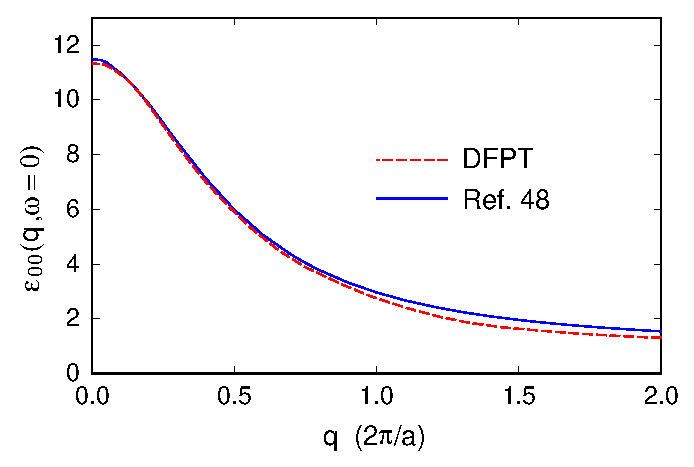
\includegraphics[width=7.5cm]{fig1.eps}
%\end    {center}
%\caption{\label{fig.pade}
%        Comparison of the dielectric function calculated for silicon 
%        on the real axis and the analytically continued function starting
%        from imaginary frequencies. The three panels correspond to the
%        cases illustrated in Fig.\ 3 of Ref.\ \onlinecite{hl86}.
%        }
%\end    {figure}

\section{Simultaneous calculation of the susceptibility at multiple frequencies}\label{app.multishift}

The linear systems Eqs.\ (\ref{eq.linsys.1.nscf}) and (\ref{eq.green.3})
can be solved efficiently by using the ``multishift'' 
cBiCG method of Ref.~\onlinecite{frommer}.
Multishift methods exploit the knowledge gained during the iterative
solution of the {\it seed system} $Ax=b$ in order to determine the solutions 
of the {\it shifted system} $Ax+\w x=b$ with only a small computational overhead.
The rationale behind such method is that the seed system and the
shifted system share the same Krilov subspaces $\{b,Ab,A^2b,\cdots\}$,
therefore the residuals of the seed and of the shifted
systems can be taken to be collinear.\cite{frommer}

This multishift technique allows us to determine the
entire frequency-dependence of the dielectric matrix
by performing one single static calculation for each set of parameters $[\q$,$\G]$ in
Eq.\ (\ref{eq.linsys.4}).
For the seed system the algorithm is still given by Eqs.\ (\ref{eq.cg1})-(\ref{eq.cg7}).
For the shifted system we replace the calculation of the residuals
$r_{n,\w}$ and of the coefficients $\alpha_{n,\w}$, $\beta_{n,\w}$ corresponding
to the frequency $\w$ by the following relations:
  \begin{equation} \label{eq.shift.1}
  r_{n,\w}  =\frac{r_n}{\pi_{n,\w}};
  \hspace{0.2cm}
  \alpha_{n,\w}  =  \frac{\pi_{n,\w}}{\pi_{n+1,\w}}\alpha_n ;
  \hspace{0.2cm}
  \beta_{n,\w}  =  \Big(\frac{\pi_{n,\w}}{\pi_{n+1,\w}}\Big)^2\beta_n,
  \end{equation}
where the scaling factor $\pi_{n+1,\w}$ is calculated through the recurrence relation
  \begin{equation}\label{eq.shift.2}
  \pi_{n+1,\w} = (1+\w\alpha_n) \pi_{n,\w} + \frac{\alpha_n\beta_{n-1}}{\alpha_{n-1}}(\pi_{n,\w}-\pi_{n-1,\w}).
  \end{equation}
In order to obtain collinear residuals $r_n$ and $r_{n,\w}$ we need to
initialize the algorithm using $x_0=0$.

The use of Eqs.~(\ref{eq.shift.1}) and (\ref{eq.shift.2}) allows us to
skip the time-consuming operations involving the Hamiltonian in
Eqs.\ (\ref{eq.cg1}) and~(\ref{eq.cg5}).
This method is extremely convienient for determining the frequency-dependent
susceptibility for many frequencies at the cost of one single calculation.

We point out that this method still carries some drawbacks.
One limitation is that this method cannot be applied to the self-consistent
system of Eq.\ (\ref{eq.linsys.1}), because the know-term on the
right-hand side depends on the frequency $\w$ itself.
Therefore the use of the shifted cBiCG method is only possible
for {\it non self-consistent calculations of the dielectric matrix}
and requires explicit matrix inversions to determine the screened
Coulomb interaction.
This approach can be regarded as an improved version 
of the technique proposed in Ref.\ \onlinecite{reining-sternheimer}.

Another limitation is that the shifted cBiCG method
does not allow for the use of preconditioners. In fact
the preconditioned seed system $M^{-1}Ax=M^{-1}b$ and the preconditioned shifted system
$M^{-1}Ax+\w M^{-1}x=M^{-1}b$ do not share the same Krilov subspaces, 
hence the residuals cannot be taken to be collinear.\cite{simoncini} 
The practical consequence is that for systems with
large basis set energy cutoffs and small band gaps, the number of iterations
required to achieve convergence could impractical.

\begin{thebibliography}{99}

\bibitem{hedin1}
L. Hedin,
Phys.\ Rev.\ {\bf 139}, A796 (1965).

\bibitem{hl86}
M. Hybertsen and S. G. Louie,
Phys.\ Rev.\ B {\bf 34}, 5390 (1986).

\bibitem{onida}
G. Onida, L. Reining, R. W. Godby, R. Del Sole, and W. Andreoni, 
Phys.\ Rev.\ Lett.\ {\bf 75}, 818 (1995).

\bibitem{rolfing}
M. Rohlfing and S. G. Louie,
Phys.\ Rev.\ B {\bf 62}, 4927 (2000).

\bibitem{reining-review}
G. Onida, L. Reining, and A. Rubio,
Rev.\ Mod.\ Phys.\ {\bf 74}, 601 (2002).

\bibitem{catalin} 
C. D. Spataru, S. Ismail-Beigi, L. X. Benedict, and S. G. Louie,
Phys.\ Rev.\ Lett.\ {\bf 92}, 077402 (2004).

\bibitem{rubio} 
K. S. Thygesen1 and A. Rubio,
Phys.\ Rev.\ B {\bf 77}, 115333 (2008).

\bibitem{catalin-lw} 
C. D. Spataru, M. A. Cazalilla, A. Rubio, L. X. Benedict, P. M. Echenique, and S. G. Louie,
Phys.\ Rev.\ Lett.\ {\bf 87}, 246405 (2001).

\bibitem{cheolhwan}
C.-H. Park, F. Giustino, M. L. Cohen, and S. G. Louie,
Nano Lett.\ {\bf XX}, XXXX (2009).

\bibitem{bruneval-oxide}
M. Gatti, F. Bruneval, V. Olevano, and L. Reining,
Phys.\ Rev.\ Lett.\ {\bf 99} 266402 (2007).

\bibitem{rinke}
P. Rinke, A. Qteish, J. Neugebauer, C. Freysoldt, and M. Scheffler, 
New J.\ Phys.\ {\bf 7}, 126 (2005). 

\bibitem{schilfegarde}
M. van Schilfgaarde, T. Kotani, and S. Faleev,
Phys.\ Rev.\ Lett.\ {\bf 96}, 226402 (2006).

\bibitem{york}
A. Schindlmayr and R. W. Godby,
Phys.\ Rev.\ Lett.\ {\bf 80}, 1702 (1998).

\bibitem{spacetime}
H. N. Rojas, R. W. Godby, and R. J. Needs,
Phys.\ Rev.\ Lett.\ {\bf 74}, 1827 (1995).

\bibitem{blochl}
S. Lebegue, B. Arnaud, M. Alouani, and P. E. Bl\"ochl,
Phys.\ Rev.\ B {\bf 67}, 155208 (2003). 

\bibitem{hl}
L. Hedin and S. Lundqvist,
Effects of the electron-electron and the electron-phonon interaction in
the one-electron states of solids,
in {\it Solid State Physics}, ed. by F. Seitz, D. Turnbull, and
H. Ehrenreich, (Academic, New York, 1969), vol.\ 23, pag. 1.

\bibitem{gunnarsson}
F. Aryasetiawan and O. Gunnarsson,
Rep.\ Prog.\ Phys.\ {\bf 61}, 237 (1998). 

\bibitem{sohrab} 
M. L. Tiago, S. Ismail-Beigi, and S. G. Louie,
Phys.\ Rev.\ B {\bf 69}, 125212 (2004).

\bibitem{bruneval-gonze}
F. Bruneval and X. Gonze,
Phys.\ Rev.\ B {\bf 78} 085125 (2008).

\bibitem{reining-sternheimer}
L. Reining, G. Onida, and R. W. Godby, 
Phys.\ Rev.\ B {\bf 56} R4301 (1997).

\bibitem{umari1}
P. Umari, G. Stenuit, and S. Baroni,
Phys.\ Rev.\ B {\bf 79}, 201104(R) (2009).

\bibitem{umari2}
P. Umari, G. Stenuit and S. Baroni,
arXiv:0910.0791.

\bibitem{gygi}
H. F. Wilson, D. Lu, F. Gygi, and G. Galli,
Phys.\ Rev.\ B {\bf 79}, 245106 (2009).

\bibitem{baroni.rmp}
S. Baroni, S. de Gironcoli, A. Dal Corso, and P. Giannozi, 
Rev.\ Mod.\ Phys.\ {\bf 73}, 515 (2001).

\bibitem{frommer}
A. Frommer,
Computing {\bf 70}, 87 (2003).

\bibitem{cohen_berg}
M. L. Cohen and T. K. Bergstresser,
Phys.\ Rev.\ {\bf 141}, 789 (1966).

\bibitem{fleszar-resta}
A. Fleszar and R. Resta,
Phys.\ Rev.\ B {\bf 31}, 5305 (1985).

\bibitem{kunc-tosatti}
K. Kunc and E. Tosatti,
Phys.\ Rev.\ B {\bf 29}, 7045 (1984).

\bibitem{giannozzi}
S. Baroni, P. Giannozzi, and A. Testa,
Phys.\ Rev.\ Lett.\ {\bf 58}, 1861 (1987).

\bibitem{degironcoli}
S. de Gironcoli,
Phys.\ Rev.\ B {\bf 51}, 6773 (1995).

\bibitem{reining94}
R. Dal Sole, L. Reining, and R. W. Godby,
Phys.\ Rev.\ B {\bf 49}, 8024 (1994).

\bibitem{espresso}
P. Giannozzi {\it et al.},
% S. Baroni, N. Bonini, M. Calandra, R. Car, C. Cavazzoni, D. Ceresoli, G. L. Chiarotti, 
%M. Cococcioni, I. Dabo, A. Dal Corso, S. Fabris, G. Fratesi, S. de Gironcoli, R. Gebauer, 
%U. Gerstmann, C. Gougoussis, A. Kokalj, M. Lazzeri, L. Martin-Samos, N. Marzari, F. Mauri, 
%R. Mazzarello, S. Paolini, A. Pasquarello, L. Paulatto, C. Sbraccia, S. Scandolo, 
%G. Sclauzero, A. P. Seitsonen, A. Smogunov, P. Umari, R. M. Wentzcovitch, 
J.\ Phys.: Condens.\ Matter {\bf 21}, 395502 (2009).

\bibitem{cpm}
R. M. Pick, M. H. Cohen, and R. M. Martin,
Phys.\ Rev.\ B {\bf 1}, 910 (1970). 

\bibitem{hl86-prb}
M. S. Hybertsen and S. G. Louie,
Phys.\ Rev.\ B {\bf 35}, 5585 (1976).

\bibitem{balde_tosa}
A. Baldereschi and E. Tosatti,
Phys.\ Rev.\ B {\bf 17}, 4710 (1978).

\bibitem{baroni-resta}
S. Baroni and R. Resta,
Phys.\ Rev.\ B {\bf 33}, 7017 (1986).

\bibitem{alavi}
J. Spencer and A. Alavi.
Phys.\ Rev.\ B {\bf 77} 193110 (2008).

\bibitem{painless.cg}
G.\ H.\ Golub and C.\ F.\ Van Loan, {\it Matrix Computations} (John Hopkins University Press, Baltimore, 1983).

\bibitem{jacobs}
D.\ A.\ H.\ Jacobs,
IMA J.\ Numer.\ Anal.\ {\bf 6}, 446 (1986).

\bibitem{tpa}
M. P. Teter, M. C. Payne, and D. C. Allan,
Phys.\ Rev.\ B {\bf 40}, 12255 (1989).

\bibitem{pade1}
K.-H. Lee and K. J. Chang,
Phys.\ Rev.\ B {\bf 54}, R8285 (1996).

\bibitem{pade2}
H. J. Vidberg and J. W. Serene,
J.\ Low.\ Temp.\ Phys.\ {\bf 29}, 179 (1977).

\bibitem{nelder-mead}
J. A. Nelder and R. Mead,
Comput. J. {\bf 7}, 308 (1965).
%We used the implementation available from the
%{\tt E04CCF} routine of the {\tt NAG} library
%({\tt www.nag.co.uk}).

\bibitem{simoncini}
V. Simoncini and D. B. Szyld,
Numer.\ Linear Algebr.\ {\bf 14}, 1 (2006).

\bibitem{frigo}
S. G. Johnson and M. Frigo,
IEEE Trans.\ Sig.\ Proc.\ {\bf 55}, 111 (2007).

\bibitem{chelikowsky}
A. Natan, A. Benjamini, D. Naveh, L. Kronik, M. L. Tiago, S. P. Beckman, and J. R. Chelikowsky,
Phys.\ Rev.\ B {\bf 78}, 075109 (2008).

\bibitem{siesta}
J. M. Soler, E. Artacho, J. D. Gale, A. Garc\`ia, J. Junquera, P. Ordej\'on, and D. S\'anchez-Portal,
J.\ Phys.: Condens.\ Matter {\bf 14}, 2745 (2002).

\end{thebibliography}

\end{document}
